\documentclass[11pt]{amsart}
\usepackage[
style=apa, natbib=true,
]{biblatex}
\addbibresource{biblio.bib} 
%prepared in AMSLaTeX, under LaTeX2e
\addtolength{\oddsidemargin}{-.65in}
\addtolength{\evensidemargin}{-.65in}
\addtolength{\topmargin}{-.5in}
\addtolength{\textwidth}{1.2in}
\addtolength{\textheight}{1.0in}
\renewcommand{\baselinestretch}{1.06}

\usepackage{wrapfig,fancyvrb,xspace}
\usepackage{palatino,bm,stmaryrd}
\usepackage[final]{graphicx}
\usepackage[pdftex, colorlinks=true, plainpages=false, linkcolor=blue, citecolor=red, urlcolor=blue]{hyperref}

% macros
\newcommand{\bn}{\mathbf{n}}
\newcommand{\bq}{\mathbf{q}}
\newcommand{\bu}{\mathbf{u}}
\newcommand{\bv}{\mathbf{v}}
\newcommand{\bw}{\mathbf{w}}
\newcommand{\bx}{\mathbf{x}}

\newcommand{\bX}{\mathbf{X}}

\newcommand{\bsigma}{\bm{\sigma}}
\newcommand{\bomega}{\bm{\omega}}

\newcommand{\cH}{\mathcal{H}}
\newcommand{\cK}{\mathcal{K}}
\newcommand{\cT}{\mathcal{T}}
\newcommand{\cV}{\mathcal{V}}

\newcommand{\dx}{\mathrm{dx}}
\newcommand{\ds}{\mathrm{ds}}

\newcommand{\RR}{\mathbb{R}}

\newcommand{\Div}{\nabla\cdot}
\newcommand{\eps}{\epsilon}
\newcommand{\grad}{\nabla}
\newcommand{\lam}{\lambda}

\newcommand{\jump}[1]{\llbracket #1 \rrbracket }


\title{Gas in a porous media, using Firedrake}
\author{Tara Shreve}
\author{Ed Bueler}
\date{\today}

\begin{document}
\maketitle
%\begin{abstract}
%FIXME
%\end{abstract}

\thispagestyle{empty}

\section{A porous medium model for Darcy-type gas flow}

Suppose $\Omega$ is a 2D or 3D domain with well-behaved boundary, such as a rectangle or other polygon in 2D, or a polyhedron in 3D.  We will use $x,y$ for the horizontal coordinates and $z$ for the vertical coordinate.  (In 2D we use only $x,z$.)  Note $z$ is measured positive upward.

Within $\Omega$ we assume there is a matrix of porous material with spatially-variable porosity $\phi(x,y,z)$ and permeability $k(x,y,z)$.  These fields are assumed independent of time, but not smooth, and in fact we will be interested in cases where they have large discontinuities.

An ideal gas flows through the medium, and we will take the properties of this gas to be positive constants: $R$ is the gas constant, $T$ is the absolute temperature, and $M$ is the molar mass.  The ideal gas law says the density $\rho$ and pressure $P$ are proportional via $c = RT/M$, a positive constant:
\begin{equation}
c \rho = P.  \label{eq:ideal}
\end{equation}

We assume that the gas flow satisfies Darcy's law \citep{Fowler2011}, thus the volumetric flux $\bq$ is driven by the gradient of the gas pressure:
\begin{equation}
\bq = - \frac{k}{\mu} \grad P \label{eq:pmtime:darcy}
\end{equation}
Here $\mu$ is the dynamic viscosity of the gas, again taken to be constant.  (For now we ignore gravity, which contributes a term \citep{Collinson2012}.)  Because mass is conserved, additionally we have:
\begin{equation}
\phi \frac{\partial \rho}{\partial t} + \Div \left(\rho\, \bq\right) = 0. \label{eq:pmtime:masscont}
\end{equation}
Here we are assuming no mass sources or sinks, as otherwise there would be an additional function on the right side.  Note that we can also write \eqref{eq:pmtime:masscont} using the (conserved) mass flux $\bsigma = \rho \bq$, with units of $\text{kg}\,\text{m}^{-2}\,\text{s}^{-1}$.  In this case the mass conservation equation is just $\partial \rho / \partial t + \Div \sigma = 0$.

Certain observations regarding these equations should be made.  First, gas density must be non-negative: $\rho\ge 0$.  Second, relative to the classic mass continuity statement ``$\partial\rho/\partial t + \Div(\rho \bv)=0$'' \citep[for example]{Tadmor2012}, where $\bv$ is the fluid velocity, note that \eqref{eq:pmtime:masscont} is scaled with the (dimensionless) porosity $\phi$.  However, $\phi$ is also implicit in the definition of $\bq$ because it is the gas volume per unit area of any face of the porous matrix: $\bq = \phi \bv$.  While the velocity $\bv$ may be helpful in understanding the solution, it is not required when stating the model.

\newcommand{\Patm}{P_{\text{atm}}}

Regarding units of the solution variables in the above equations, $\rho(t,x,y,z)$ is in SI units of $\text{kg}\,\text{m}^{-3}$, $P(t,x,y,z)$ in $\text{Pa} = \text{N}\,\text{m}^{-2}$, and $\bq(t,x,y,z)$ in $\text{m}^3\,\text{m}^{-2}\,\text{s}^{-1} = \text{m}\,\text{s}^{-1}$.  Also the porosity $\phi$ is a dimensionless ratio of volumes, thus $0\le \phi \le 1$, the permeability $k$ is in $\text{m}^2$, the constant $c$ is in $\text{J}\,\text{kg}^{-1}$, and the dynamic viscosity $\mu$ is in $\text{Pa}\,\text{s}$.

Considering the system of equations \eqref{eq:ideal}--\eqref{eq:pmtime:masscont}, it is straightforward to eliminate the pressure $P$ and flux $\bq$, if this is desired:
\begin{equation}
\phi \frac{\partial \rho}{\partial t} - \Div \left(\frac{k}{\mu} \rho \grad\left(c \rho\right)\right) = 0. \label{eq:pmtime:primal}
\end{equation}
This form is comparable to the better-known heat equation
\begin{equation}
\frac{\partial u}{\partial t} - \Div(\grad u) = 0. \qquad \text{\emph{(heat equation)}}\label{eq:heattime:primal}
\end{equation}
An important property of \eqref{eq:heattime:primal} is that the operator $\Div \grad = \grad^2$ acts as an invertible matrix when finding the solution $u$.  However, since $\rho$ appears as a flux coefficient in \eqref{eq:pmtime:primal}, invertibility is lost in \eqref{eq:pmtime:primal} if $\rho\to 0$ somewhere.  Such ``degeneration'' of the diffusivity is a well-known concern with the porous medium equation \eqref{eq:pmtime:primal} \citep[for example]{Vazquez2007}, and it will influence the numerical solution method below.

The models above are time dependent, but setting $\partial \rho/\partial t = 0$ yields the steady-state version of the porous medium equation, here written in terms of the conserved mass density $\rho$:
\begin{equation}
- \Div\left(\frac{k}{\mu} \rho \grad\left(c \rho\right)\right) = 0
\label{eq:pm:strong}
\end{equation}

Suitable boundary conditions must be applies to \eqref{eq:pm:strong}.  On the ``Dirichlet'' part of the boundary, denoted $\Gamma_D \subset \partial\Omega$, the density is given by a continuous function $\rho_D(x,y,z)$.  Equivalently the pressure may be given on $\Gamma_D$.  On the remainder of the boundary $\Gamma_N = \partial\Omega \setminus \Gamma_D$, the ``Neumann'' boundary, the normal mass flux is zero:
\begin{subequations}
\label{eq:strongbcs}
\begin{align}
\rho|_{\Gamma_D}               &= \rho_D \\
(\bsigma\cdot \bn)|_{\Gamma_N} &= 0
\end{align}
\end{subequations}
It is straightforward to extend the model with provided values of the mass flux, i.e.~$(\bsigma\cdot \bn)|_{\Gamma_N}= \sigma_N$ where $\sigma_N$ is given, for a non-homogeneous Neumann condition.  System \eqref{eq:pm:strong} with boundary conditions \eqref{eq:strongbcs} apparently forms a well-posed problem as long as $\Gamma_D$ has positive measure (within $\partial\Omega$) and $\rho_D\ge 0$.  In the time-dependent case, classical solutions exist if additionally $\rho_D$ is actually positive and the initial density is positive \citep[Theorem 3.1]{Vazquez2007}.

The equations above form a nonlinear model for the density $\rho$, with degeneration of the diffusivity if $\rho \to 0$.  However, a straightforward substitution allows us to rewrite the problem as a linear diffusion problem.  Let
\begin{equation}
u = \rho^2 \label{eq:pm:defu}
\end{equation}
and define convenience constant $\alpha = c/(2\mu)$.  Then \eqref{eq:pm:strong}, \eqref{eq:strongbcs} becomes
\begin{subequations}
\label{eq:pm:strongu}
\begin{align}
- \alpha \Div\left(k \grad u \right) &= 0 & &\text{on } \Omega \label{eq:pm:strongu:eqn} \\
u &= \rho_D^2 & &\text{on } \Gamma_D  \label{eq:pm:strongu:bcD} \\
\grad u \cdot \bn &= 0 & &\text{on } \Gamma_N  \label{eq:pm:strongu:bcN} 
\end{align}
\end{subequations}
The (mixed) strong-form system \eqref{eq:pm:strongu} is a steady-state, semi-linear advection-diffusion problem for the squared density $u$.  The density $\rho$ and pressure $P$ are easily recovered via \eqref{eq:pm:defu}, \eqref{eq:ideal} as long as the solution satisfies $u\ge 0$.


\section{Weak form and FE method (for discontinuous permeability)}

In this section we derive the weak form which is needed for an FE method.  The method we use is conforming, that is, it finds a continuous approximate solution living in the same function space where the continuum solution lives.  Both the continuum and FE solutions solve the same weak form, though the latter is over a smaller, finite-dimensional subspace.

Recall that $H^1(\Omega)$ denotes the Sobolev (Hilbert) space of functions on $\Omega$ with weak derivatives which are square-integrable functions \citep[chapter 5]{Evans2010}, and write $H_0^1(\Omega)$ for the subspace of $H^1(\Omega)$ which have zero trace along $\Gamma_D$.  We multiply the strong form equation \eqref{eq:pm:strongu:eqn} by a test function $v \in H_0^1(\Omega)$.  For a scalar function $f$ and a vector field $\bX$, recall the divergence theorem $\int_\Omega \Div \bX\,\dx = \int_{\partial \Omega} \bX\cdot \bn\,\ds$ and the product rule $\Div(f\bX) = \grad f \cdot \bX + f \Div \bX$.  Using these tools, integration by parts generates
\begin{equation}
\int_\Omega \alpha k \grad u \cdot \grad v\,\dx - \int_{\partial\Omega} k v \grad u \cdot \bn\,\ds = 0 \label{eq:weaku:early}
\end{equation}
Since $v\in H_0^1(\Omega)$, the portion of the boundary integral which is in $\Gamma_D$ is zero, and \eqref{eq:pm:strongu:bcN} implies that the remaining integral over $\Gamma_N$ is zero.  Thus 
\begin{equation}
\int_\Omega \alpha k \grad u \cdot \grad v\,\dx = 0. \label{eq:weaku}
\end{equation}

While our FE method will follow a standard approach to Poisson equations, it is worth considering the theoretical setting for \eqref{eq:weaku}, especially because we will solve cases where the permeability field $k(x,y,z)$ has discontinuous jumps.  First, we assume that $k\in L^\infty(\Omega)$ with a positive lower bound; there is $k_0>0$ so that $k \ge k_0$.  Such a lower bound implies that the operator $L w = - \Div(k \grad w)$ is uniformly elliptic \citep[section 6.1]{Evans2010}.  We will assume that the boundary value $u_D = \rho_D^2$, defined only on $\Gamma_D$, is the trace of some $g\in H^1(\Omega)$, so that if $u\in H^1(\Omega)$ then $\tilde u = u - g \in H_0^1(\Omega)$.  The theory of problem \eqref{eq:weaku} then shows that there is a unique weak solution $u\in H^1(\Omega)$.  Specifically, apply Theorem 3 in section 6.2 of \citep{Evans2010}, noting the comments on pages 315 and 322, regarding boundary values and the constant in the Poincare inequality, respectively.  It is this weak solution of \eqref{eq:weaku} which we are seeking to approximate, and indeed the earlier strong form \eqref{eq:pm:strongu:eqn} generally will not have a solution so that the repeated (i.e.~second) derivative in that equation is actually meaningful.

FIXME The permeability field $k(x,y,z)$ may be discontinuous, but for the purposes of the following FE method we will assume that the element faces (edges in 2D) include any of its discontinuities.  (In other words, we assume the mesh is adapted to any permeability discontinuities.)

FIXME integrate over domains where $k$ is constant, and observe that the solution of this weak form has jump integrals which are zero

FIXME Next we assume that the mesh (triangulation) $\cT_h$ exactly covers the domain: $\bigcup_{E\in\cT_h} \bar E = \bar \Omega$.

FIXME The density $\rho$ and pressure $P$ are recovered from $u$ via \eqref{eq:pm:defu} and \eqref{eq:ideal}.


\section{Firedrake implementation and solution}

To implement the above in Firedrake we must choose a finite element space $u$, which we take to be a space of $C^0$ piecewise-polynomial functions of degree $j$, namely $\text{CG}_j$ \citep{Elman2014}.  On $\Gamma_D$ we must impose the essential requirement that $u=\rho_D^2$ on the solution, and $v=0$ on the test functions, and this is done through Firedrake's \verb|DirichletBC()| command.
\begin{Verbatim}[fontsize=\small,frame=lines]
H = FunctionSpace(mesh, 'CG', j)
u = Function(H, name='u (rho^2)')
v = TestFunction(H)
\end{Verbatim}
Weak form \eqref{eq:weaku} then corresponds to the UFL code
\begin{Verbatim}[fontsize=\small,frame=lines]
alf = c / (2.0 * mu)
F = alf * k * dot(grad(u), grad(v)) * dx(degree=4)
\end{Verbatim}
The quadrature degree is fixed so as to disable Firedrake's automatic quadrature degree mechanism, which can generate unstable and inefficient degrees which are too large.

We solve the equations by a sparse direct matrix method \citep{Amestoy2001}:
\begin{Verbatim}[fontsize=\small,frame=lines]
solve(F == 0, u, bcs=[BCs,],
      solver_parameters = {'snes_type': 'ksponly',
                           'ksp_type': 'preonly',
                           'pc_type': 'lu',
                           'pc_factor_mat_solver_type': 'mumps'})
\end{Verbatim}
A more advanced iterative, block-wise, and multigrid solver is possible \citep[e.g.][]{Bueler2021}, but it will require careful development.


\section{An application for gas flow through a porous lava dome}

In \cite{Graham2023}, we measure permeability of samples from various textural units of the Obsidian dome and South Deadman dome using field and lab permeameters. These two domes are silicic lava flows in the Inyo Craters portion of the Mono-Inyo Craters in eastern California, a chain of silicic lava flows, domes, and explosion craters that stretches 12 km (7.5 miles) to the north-northeast of Long Valley Caldera. The Inyo craters erupted as recently as ~675 years (~1350 A.D.) before present. Prior studies subdivided the majority of the lava erupted at the Inyo Craters according to the observed vesicle textures found in different parts of each flow, subdivided into finely vesicular pumice (FV), coarsely vesicular pumice (CV), and dense obsidian (OB). Shallow scientific bore hole drilling in the 1970's confirmed the presence of an underground magmatic intrusion, which was the source of the domes. This drilling also provided some general constraints on the depth of each distinct textural unit within the dome (Table \ref{tab:UnitPermPoro}).

In this study, we wish to put constraints on the surface gas flux for each textural unit at Obsidian Dome. The unit mapping of the dome is shown in Fig. \ref{fig:unitMapping}, and an example cross-section is shown in Fig. \ref{fig:crossSection}. Using constraints on dome height, the depth and permeability of each unit, and assuming a significant portion of gas is sourced from degassing of the underlying feeder dike, we can use Darcy's law to calculate the surface gas flux through each unit. This was done in \cite{Graham2023} using a 1D model of Darcy's law, as implemented in \cite{Edmonds2003}, and we wish to extend this model into 2-dimensions, to account for the unit layering, which may affect the path of gas flow towards the surface.

COMSOL model results for gas density and surface gas flux are shown in Fig. \ref{fig:COMSOLresults}, with annotations stating relevant boundary conditions. Here we assume atmospheric pressure at the surface ($P_{atm} = 1.01325$ bar) and a pressure at the base of the dome ($L=22$ m) of $P_{z=L} = 11$ bar. There is a gas inlet at the base of the CV unit, through which steam at a temperature of 920$^{\circ}$C can enter the dome porous matrix. For simplicity, a no flow condition is imposed at the unit sides, and we choose to solve for the steady-state isothermal, compressible gas flow using Darcy's Law to relate volumetric gas flux and pressure. The porosity and permeability for each unit, as well as their height and percent of total dome surface area, are shown in Table \ref{tab:UnitPermPoro}.

\begin{figure}
   \centering
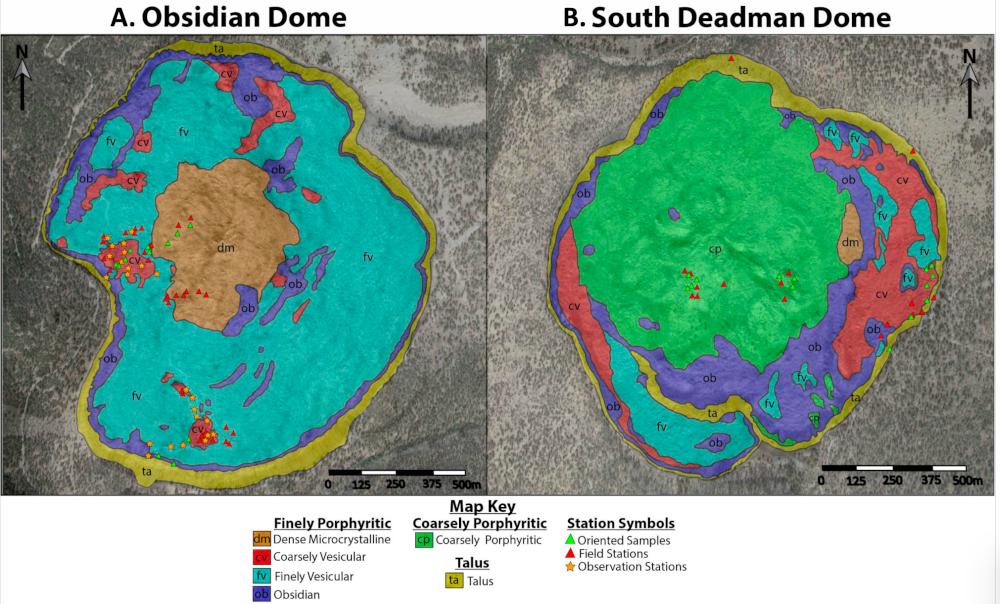
\includegraphics[width=0.95\textwidth]{figs/unitMapping-small.png}
\caption{Textural lithologic distribution maps of lavas for (A) Obsidian dome and (B) South Deadman dome.}
\label{fig:unitMapping}
\end{figure}

\begin{figure}
   \centering
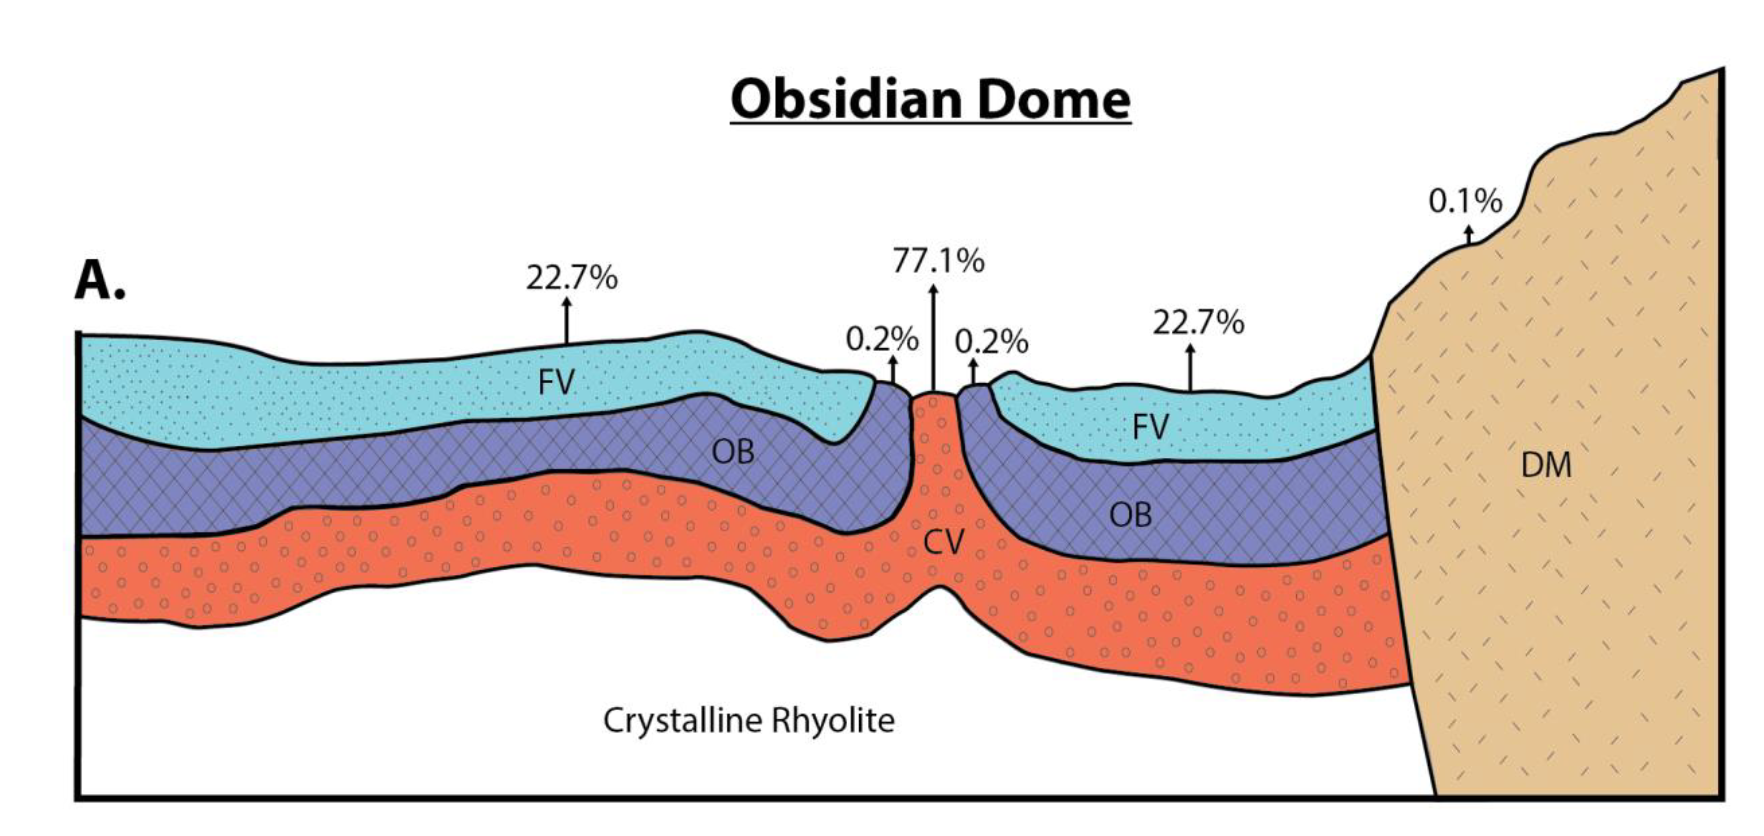
\includegraphics[scale=0.5]{figs/crossSection.png}
\caption{Schematic diagrams depicting total calculated gas flux percentages during the final stages of lava emplacement at Obsidian dome. Total gas flux for each lithologic unit was calculated using the gas flux model of Edmonds et al. (2003), and the gas flux percentages represent the percent gas flux for each lithologic unit relative to the total gas flux calculated for all units, and does not consider additional degassing that occurs through conduit processes, fractures, tuffisite veins, or porous pathways that are too large to measure.}
\label{fig:crossSection}
\end{figure}

\begin{figure}
   \centering
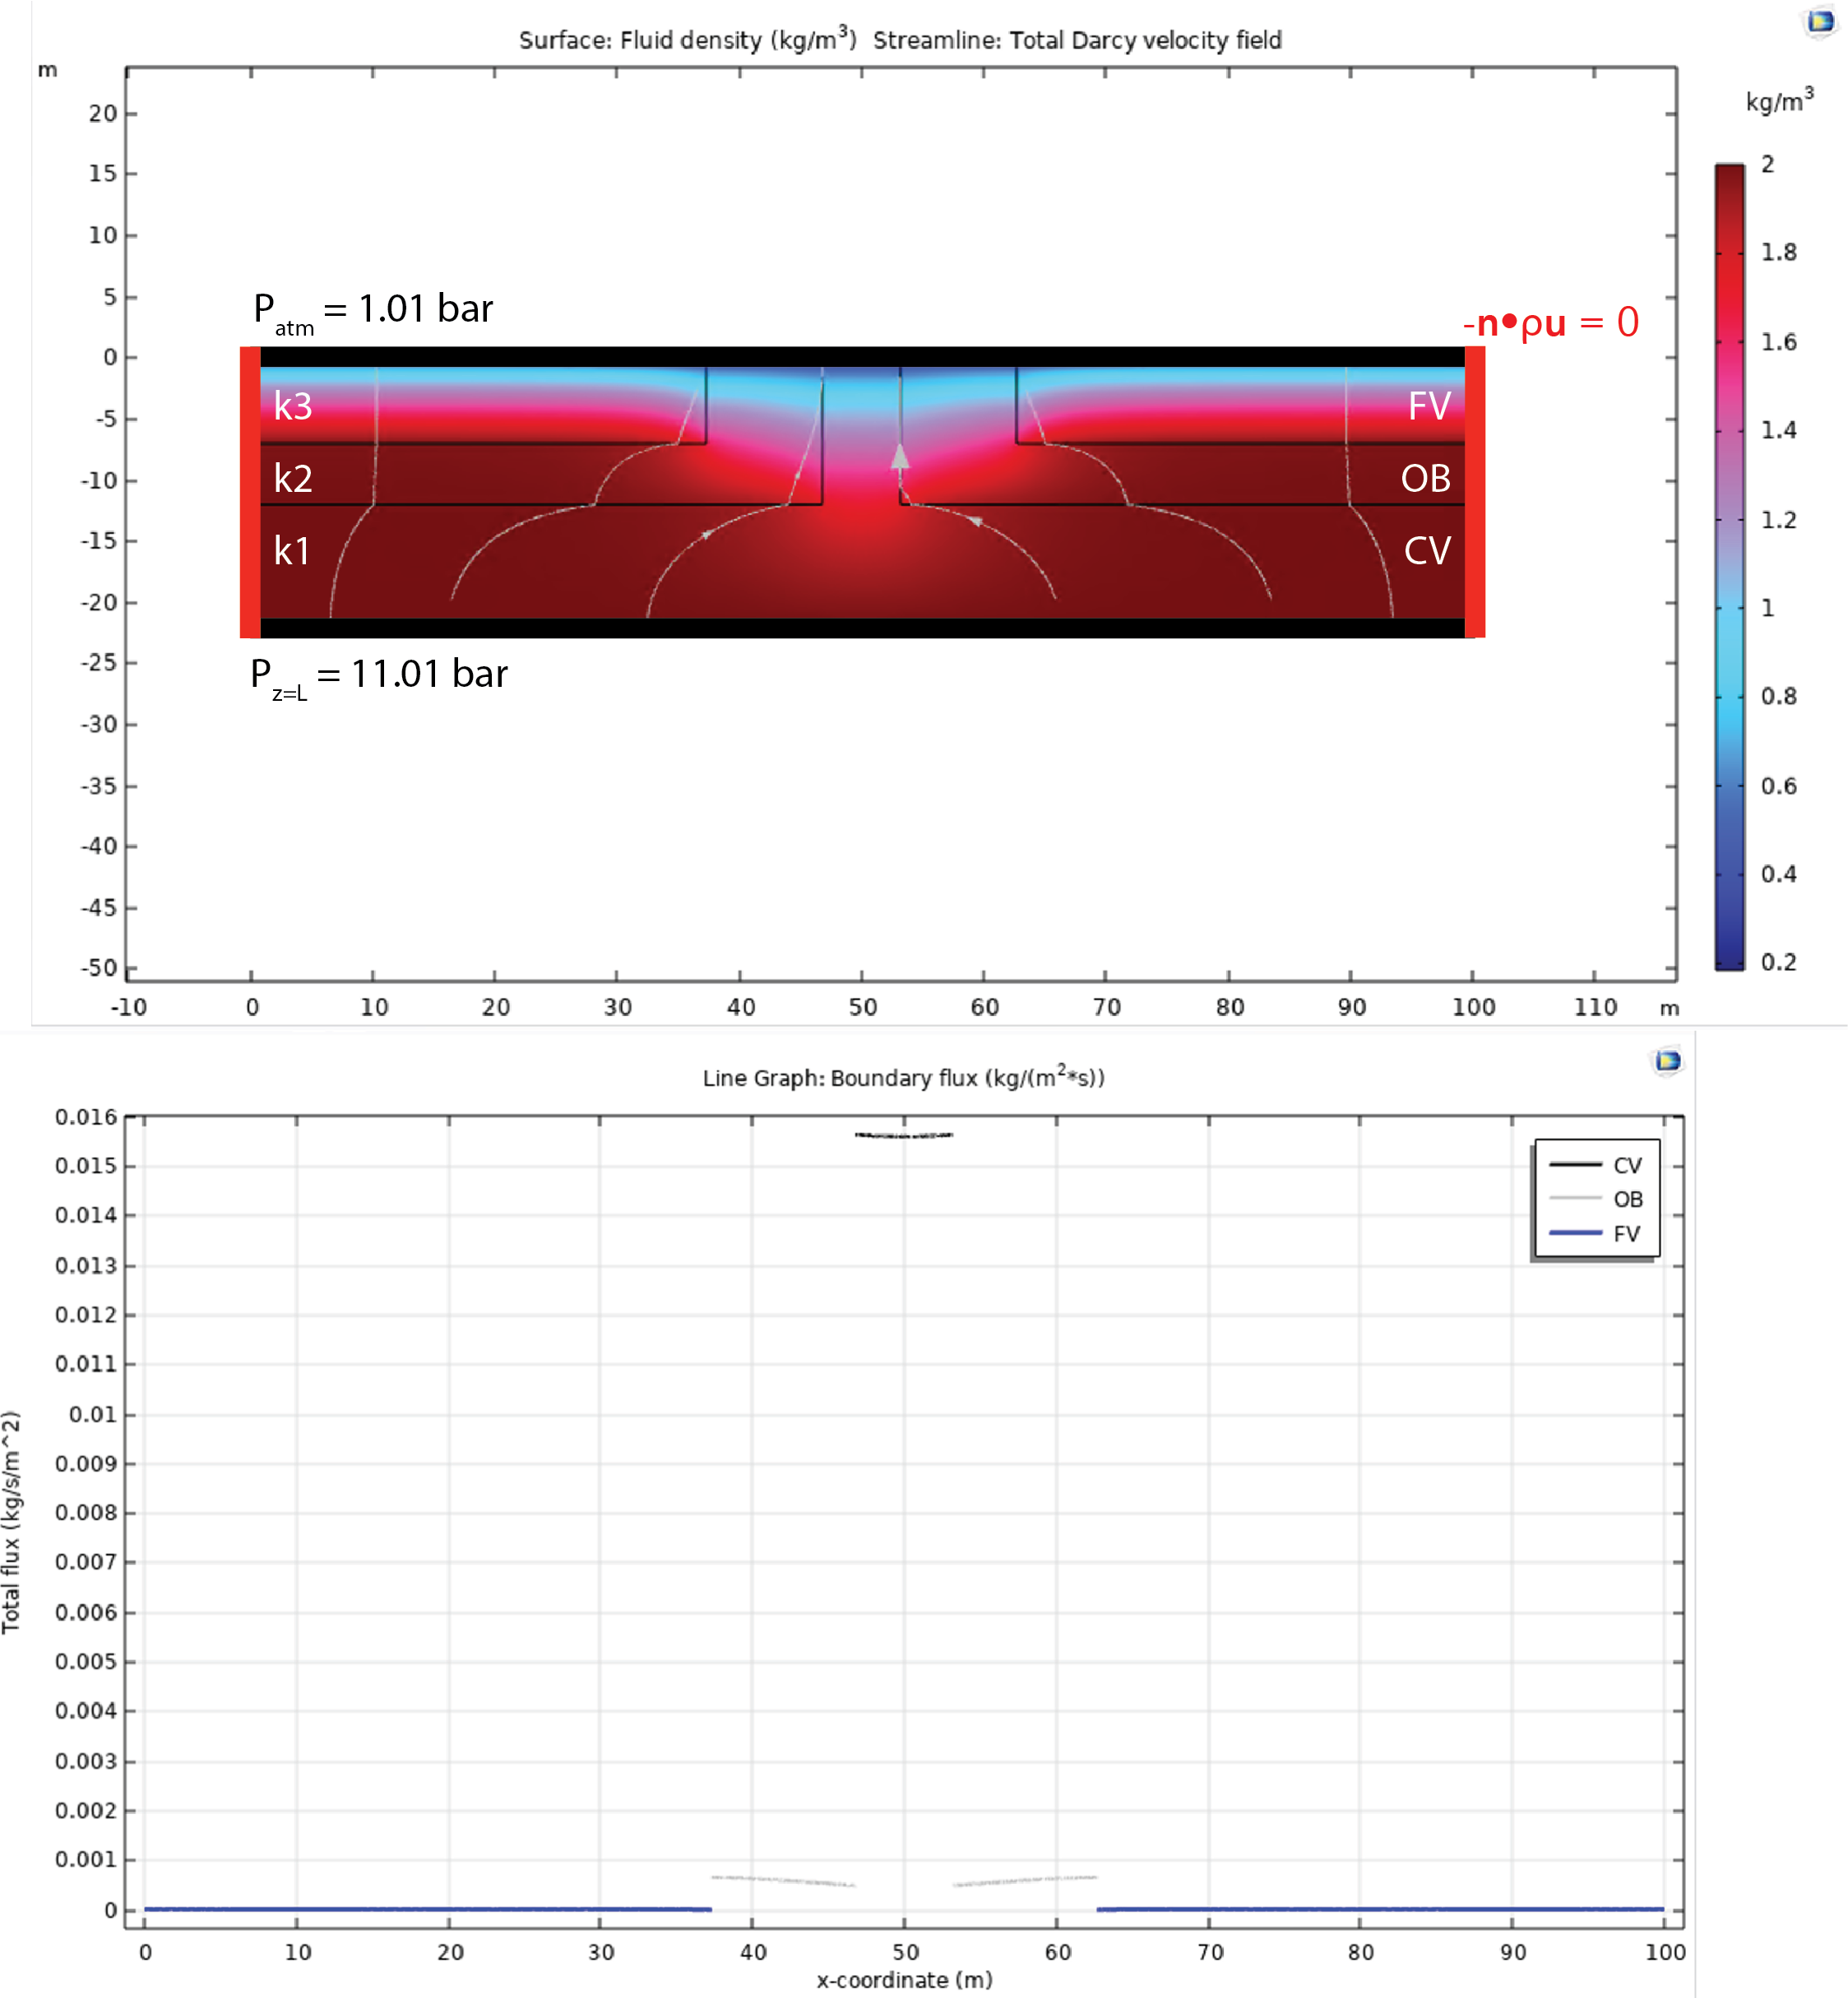
\includegraphics[scale=0.8]{figs/comsolDarcyLaw_units.png}
\caption{Top figure shows gas density in unit layers CV, FV, and OB, with permeabilities k1, k2, and k3, respectively (see Table \ref{tab:UnitPermPoro}). Streamlines indicate the direction of gas flow. Pressure boundary conditions at the base and surface of the units are shown in black, and no flow boundary conditions at the side of the units are shown in red. The bottom figure shows the gas flux at the surface.}
\label{fig:COMSOLresults}
\end{figure}


\begin{table}[h]
\center
      \small
      \begin{tabular}{lllll}
      \hline
      \textbf{Unit} & \textbf{Permeability (m\textsuperscript{2})} & \textbf{Connected porosity (\%)}  & \textbf{Height (m)} & \textbf{Percent of total dome surface area} \\  
      \hline
      CV & 6.87E-12 & 50.0 & 10 & 6.4 \\
      FV & 2.18E-13 & 23.2 &  7 & 74.6 \\
      OB & 4.94E-15 & 3.24 & 5 & 19.0 \\ 
\end{tabular}%}
\caption{Average permeability, porosity, height, and percent of total dome surface area of each textural unit.} 
\label{tab:UnitPermPoro}
\end{table}

\printbibliography

\end{document}
